%%%%%%%%%%%%%%%%%%%%%%%%%%%%%%%%%%%%%%%%%
% 
% LaTeX Template
% Version 3.1 (25/3/14)
%
%%%%%%%%%%%%%%%%%%%%%%%%%%%%%%%%%%%%%%%%%

%----------------------------------------------------------------------------------------
%	PACKAGES AND DOCUMENT CONFIGURATIONS
%----------------------------------------------------------------------------------------

\documentclass[12pt, a4 paper]{article}

\usepackage{tikz}
%\usepackage[top=2cm, bottom=2cm, outer=0cm, inner=0cm]{geometry}
\usepackage{graphicx} % Required for the inclusion of images
\usepackage{multicol} % Required for multicolumns
\usepackage{setspace} % Required for line spacing
\setlength\parindent{0pt} % Removes all indentation from paragraphs
\setlength{\columnseprule}{0.4pt} % Adds vertical line between multicolumns
\usepackage{multirow} % Required for multirows
\usepackage{booktabs} % For prettier tables
\usepackage{ragged2e}
\usepackage{xcolor}
%\usepackage{tabularx}
%\renewcommand{\rmdefault}{ptm}

%\usepackage{helvet}

\usepackage{times} % Uncomment to use the Times New Roman font

%----------------------------------------------------------------------------------------
%	DOCUMENT INFORMATION
%----------------------------------------------------------------------------------------

\begin{document}

\tikz[remember picture,overlay] \node[inner sep=0pt] at (current page.center){
\includegraphics[width=\paperwidth,height=\paperheight]{image1.png}};

\clearpage

%\font\myfont=cmr12 at 35pt
%\title{\myfont  Event Name} % Write Event name here
%\author{}
%\date{\vspace{-10ex}}

%\maketitle % Insert the title, author and date
\setstretch{1}

\tikz[remember picture,overlay] \node[opacity=0.8,inner sep=0pt] at (current page.center){
\includegraphics[width=\paperwidth,height=\paperheight]{Border48-A4--Arvin61r58.png}};
%\tikz[remember picture,overlay] \node[opacity=0.5,inner sep=0pt] at (current page.center){\includegraphics[width=\paperwidth,height=\paperheight]{color-2174049__340.png}};

\begin{center}
\Huge \bfseries \ttfamily APTITUDE QUIZ
\end{center}

\begin{center}
\large A test based on technical questions
\end{center}

\begin{center}
\begin{multicols}{2}
\begin{tabular}{l r}
Date: & 08/04/2019\\ % Date the event was held
Time: & 3 P.M onwards \\ % Time of event 
\end{tabular}
\columnbreak
\begin{tabular}{l c}
Venue: & Mechanical Seminar Hall \\ % Venue of event
Total Attendance: & 86\\ % Number of participants
\end{tabular}
\end{multicols}

\bigskip

\begin{large}
%\begin{multicols}{2}
\justify
A Quiz based event ‘TECHNICAL APTITUDE QUIZ’ was organized by ISTE(INDIAN SOCIETY FOR TECHNICAL EDUCATION) in collaboration with SCIE and E2S2 on April 8,2019 in Mechanical Seminar Hall. 

\justify
It was the first round –Selection Round for the Technical Aptitude Quiz.

\justify
The event was mainly organized to test and improve the Aptitude of the students. The top 10participants were selected for the ‘Second Round of TECHNICAL APTITUDE QUIZ’. 

\justify
In the Selection Round the participants were provided with a set of 25 questions, which they were required to wind up in exact 25 minutes. Giving them one minute per question.
 
\newpage
\justify
The cut o ff for the next round of ‘Technical Aptitude Quiz’ was set to be above score 15/25. Those 9 students whose score fit the criteria were promoted to the Round 2.


\justify
The second round of ‘Technical Aptitude Quiz’ was the Qualifying Round, the selected students were provided with a set of 15 questions and were allotted a time of 10 minutes. The usage of cell phones was prohibited, neither the participants were allowed to discuss while the quiz was going on.
 

\end{large} 
\end{center}

\tikz[remember picture,overlay] \node[opacity=0.8, inner sep=0pt] at (current page.center){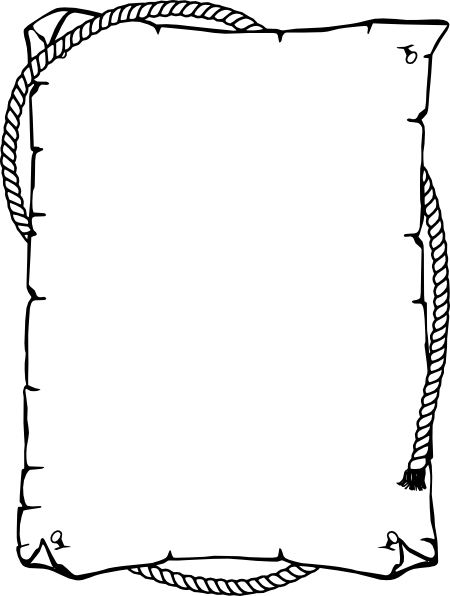
\includegraphics[width=\paperwidth,height=\paperheight]{5TRrp44jc.png}};
%\tikz[remember picture,overlay] \node[opacity=0.8,inner sep=0pt] at (current page.center){\includegraphics[width=\paperwidth,height=\paperheight]{md_5b0912b7c0870.png}};

\newpage

\tikz[remember picture,overlay] \node[opacity=0.8, inner sep=0pt] at (current page.center){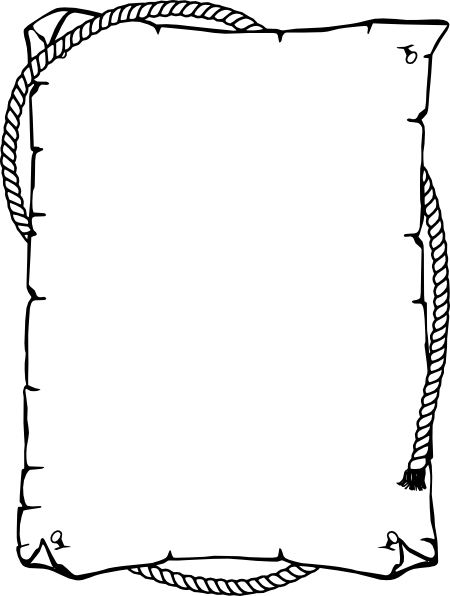
\includegraphics[width=\paperwidth,height=\paperheight]{5TRrp44jc.png}};

\begin{center}
\Huge Pictures Section

\medskip

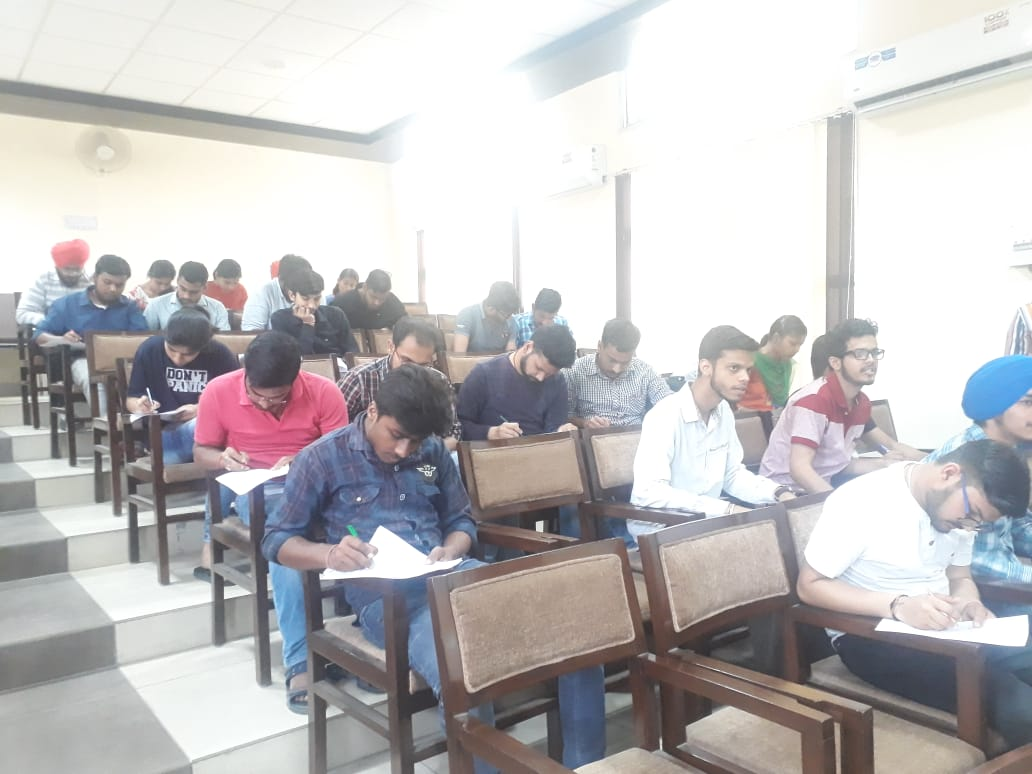
\includegraphics[height=6cm]{image2.jpg}
\medskip

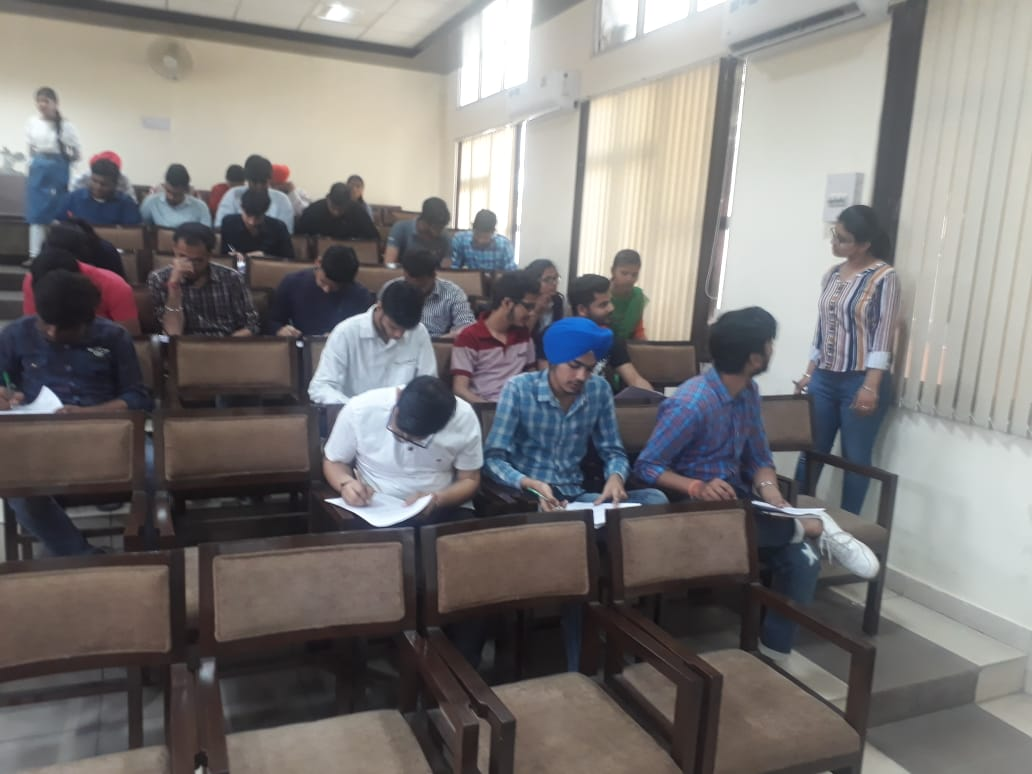
\includegraphics[height=6cm]{image3.jpg}
\medskip

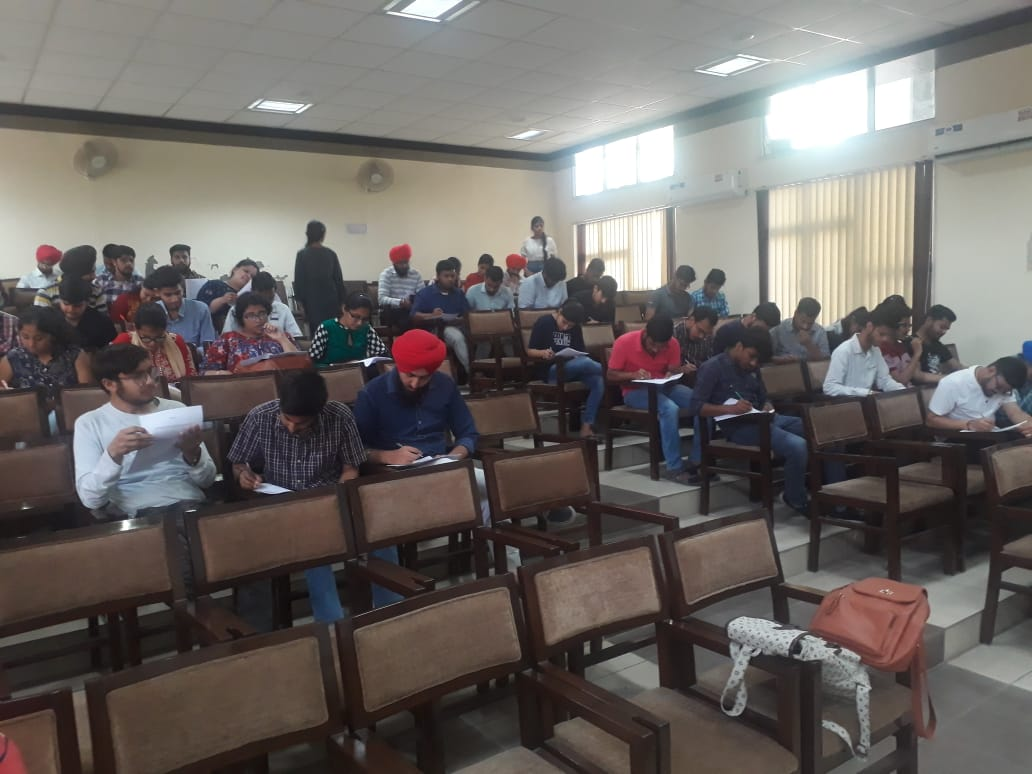
\includegraphics[height=6cm]{image4.jpg}
\begin{center}

\end{center}

\newpage

\huge Organisers list
\end{center}

\begin{table}[h!]
  \begin{center}
    \begin{tabular}{|c|c|c|c|c|c|} 
    \toprule % <-- Toprule here
      \textbf{S.No.} & \textbf{Name} & \textbf{Branch/Year} & \textbf{Roll No.} \\
      \midrule % <-- Midrule here
      1 & KIRT PREET SINGH & D2 ECE	& 1706741 \\
      2	& TUSHAR CHAUHAN   & D2 ME	& 1706533 \\
      3	& MANPREET	       & D2 CSE	& 1706471 \\
      4	& ALOK	           & D2 ME	& 1706945 \\
      5	& PAWANDEEP SINGH  & D4 CSE	& 1507637 \\
      6	& JATIN TYAGI	   & D4 ECE	& 1507883 \\
      7	& BINAY RANJAN	   & D4 ME	& 1508229 \\
      8	& VISHAL RAJ	   & D3 PE	& 1607467 \\

      \bottomrule % <-- Bottomrule here
    \end{tabular}
  \end{center}
\end{table}


\tikz[remember picture,overlay] \node[opacity=0.8,inner sep=0pt] at (current page.center){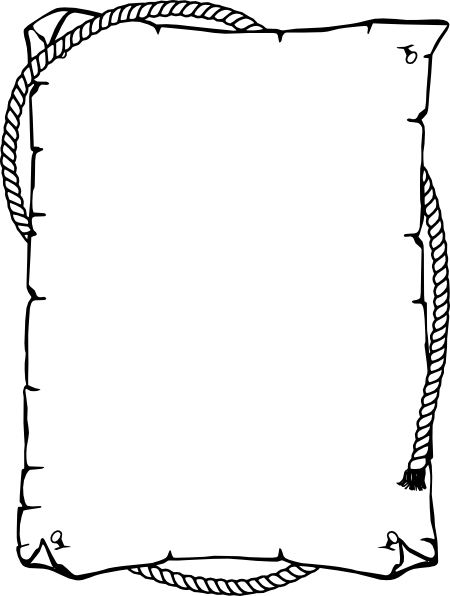
\includegraphics[width=\paperwidth,height=\paperheight]{5TRrp44jc.png}};
%\tikz[remember picture,overlay] \node[opacity=0.8,inner sep=0pt] at (current page.center){\includegraphics[width=\paperwidth,height=\paperheight]{md_5b0912b7c0870.png}};

\begin{center}
\huge Winners List
\end{center}

\begin{table}[h!]
  \begin{center}
    \begin{tabular}{|c|c|c|c|c|c|} 
    \toprule % <-- Toprule here
      \textbf{S.No.} & \textbf{Name} & \textbf{Branch/Year} & \textbf{Roll No.} &\textbf{Position} \\
      \midrule % <-- Midrule here
      1 & HARSHIT	    & D3 EE	 & 1606823 & 1st \\
      2	& HARDEEP SAINI	& D3 EE	 & 1606852 & 2nd \\
      3	& ACHINTYA	    & D2 CSE & 1706390 & 3rd \\

      \bottomrule % <-- Bottomrule here
    \end{tabular}
  \end{center}
\end{table}

\newpage
\tikz[remember picture,overlay] \node[opacity=0.8,inner sep=0pt] at (current page.center){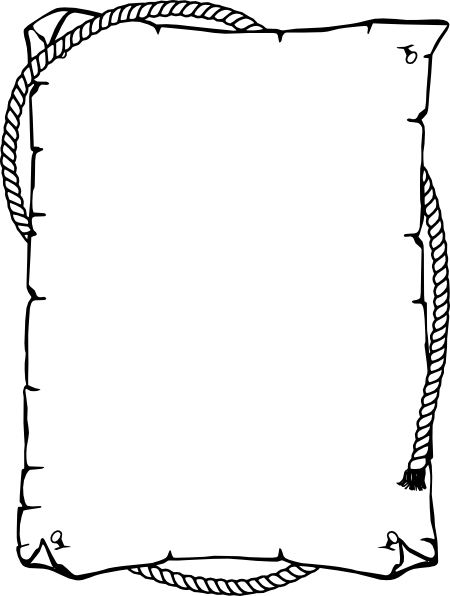
\includegraphics[width=\paperwidth,height=\paperheight]{5TRrp44jc.png}};
%\tikz[remember picture,overlay] \node[opacity=0.8,inner sep=0pt] at (current page.center){\includegraphics[width=\paperwidth,height=\paperheight]{md_5b0912b7c0870.png}};

\begin{center}
\huge Participants List
\end{center}

\begin{table}[h!]
  \begin{center}
    \begin{tabular}{|c|c|c|c|c|c|} 
    \toprule % <-- Toprule here
      \textbf{S.No.} & \textbf{Name} & \textbf{Branch} & \textbf{Year} &\textbf{Roll No.} \\
\midrule % <-- Midrule here
1       &Varun Sharma   &ME     &3rd    &1707157\\
2       &Ritesh Kutlehria       &ME     &3rd    &1707148\\
3       &Sukhdeep Singh &ME     &3rd    &1607360\\
4       &Sunil  &ME     &3rd    &1607363\\
5       &Sagar  &ME     &3rd    &1707150\\
6       &Vipin  &ME     &3rd    &1707158\\
7       &Suraj Kumar    &ME     &3rd    &1607465\\
8       &Pardeep Singh  &ME     &3rd    &1607451\\
9       &Anmol Puri     &C.E.   &2nd    &1714150\\
10      &Shiv Shankar   &ECE    &3rd    &1607025\\
11      &Achintya       &CSE    &2nd    &1706390\\
12      &Aditya &EE     &1st    &1816005\\
13      &Aditya Kumar   &EE     &1st    &1816006\\
14      &Deepak Singh   &EE     &1st    &1816023\\
15      &Vishal Kumar Verma     &ME     &3rd    &1607381\\
16      &Ashutosh       &CSE    &1st    &1808165\\
17      &Jaspreet Singh &EE     &3rd    &1606862\\
18      &Akshit Sharma  &EE     &3rd    &1606823\\
19      &Akshit &CSE    &1st    &1815004\\
20      &Guneet Kohli   &CSE    &1st    &1805172\\
21      &Divneet        &CSE    &1st    &1805169\\
22      &Arshdeep       &CSE    &1st    &1805961\\
23      &Priyanka       &EE     &1st    &1805321\\
24      &Jashanpreet    &CSE    &1st    &1805188\\
25      &Mayank Bakshi  &EE     &2nd    &1819955\\
26      &Sakshi Priya   &EE     &1st    &1805337\\
27      &Ravneet Kaur   &EE     &1st    &1805323\\
28      &Ujwal Sood     &ME     &1st    &1805720\\
29      &Himanshu Singh &ME     &1st    &1805653\\
30      &Rajat Sharma   &CE     &1st    &1805092\\
 \bottomrule % <-- Bottomrule here
    \end{tabular}
  \end{center}
\end{table}

\newpage
\tikz[remember picture,overlay] \node[opacity=0.8,inner sep=0pt] at (current page.center){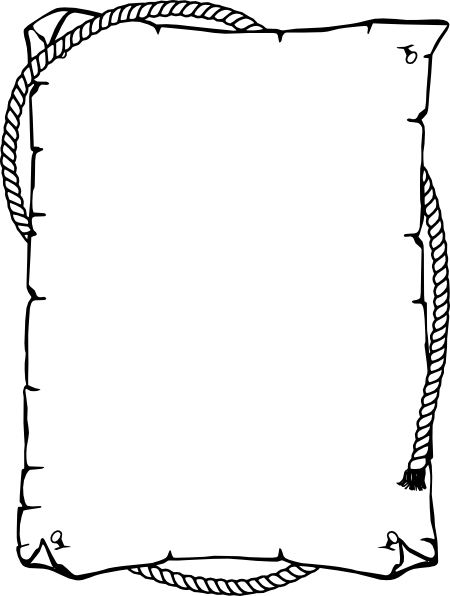
\includegraphics[width=\paperwidth,height=\paperheight]{5TRrp44jc.png}};

\begin{table}[h!]
  \begin{center}
    \begin{tabular}{|c|c|c|c|c|c|} 
    \toprule % <-- Toprule here
      \textbf{S.No.} & \textbf{Name} & \textbf{Branch} & \textbf{Year} &\textbf{Roll No.} \\
\midrule % <-- Midrule here
31      &Vishal Das     &CE     &1st    &1805122\\
32      &Paramjit Singh &CSE    &3rd    &1706562\\
33      &Ayush Gautam   &CE     &2nd    &1805129\\
34      &Nikita Gulati  &CSE    &4th    &1507630\\
35      &Simranjit Kaur &CSE    &3rd    &1706524\\
36      &Akshay Seni    &ME     &2nd    &1706945\\
37      &Sahil Gupta    &ME     &2nd    &1707056\\
38      &Jagmeet Singh  &ECE    &2nd    &1706728\\
39      &Shashi Bhushan &ECE    &3rd    &1607023\\
40      &Shubam Kumar Singh     &ECE    &3rd    &1607030\\
41      &Ujjwal Kumar   &ECE    &3rd    &1607034\\
42      &Sanjay Kumar   &ECE    &3rd    &1607022\\
43      &Priyanka Kumari        &ECE    &3rd    &1706807\\
44      &Divya Bharti   &ECE    &3rd    &1706797\\
45      &Gurpreet Kundal        &EE     &3rd    &1606850\\
46      &Hardeep Saini  &EE     &3rd    &1606852\\
47      &Neha Dwivedi   &EE     &3rd    &1706691\\
48      &Rahul Kumar    &ECE    &3rd    &1706809\\
49      &Subhash Kumar  &ECE    &3rd    &1706812\\
50      &Sachin Chandel &EE     &3rd    &1706693\\
51      &Abhishek Goyal &EE     &3rd    &1706672\\
52      &Manik Walia    &EE     &3rd    &1706688\\
53      &Gurpartap Singh        &EE     &3rd    &1706680\\
54      &Gurpreet Kaur  &CSE    &3rd    &1606678\\
55      &Jasmeet Singh  &CSE    &3rd    &1706551\\
56      &Jaspreet Kaur  &CSE    &3rd    &1706552\\
57      &Vinayak        &CSE    &2nd    &1706538\\
58      &Aman Chauhan   &CSE    &1st    &1805158\\
59      &Pawan Kumar    &ECE    &1st    &1805429\\
60      &Uday Prakash   &ME     &3rd    &1607372\\
61      &Gurjot Singh   &IT     &4th    &1507913\\
62      &Nitya Garg     &CSE    &4th    &1507634\\
63      &Alok Kumar Singh       &EE     &3rd    &1606825\\
64      &Manish Kumar   &CE     &3rd    &1614376\\
65      &Aditya Bhardwaj        &ME     &3rd    &1607202\\
\bottomrule % <-- Bottomrule here
    \end{tabular}
  \end{center}
\end{table}

\newpage
\tikz[remember picture,overlay] \node[opacity=0.8,inner sep=0pt] at (current page.center){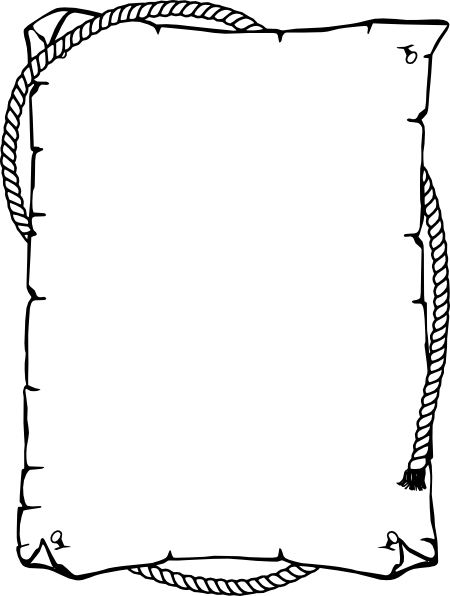
\includegraphics[width=\paperwidth,height=\paperheight]{5TRrp44jc.png}};

\begin{table}[h!]
  \begin{center}
    \begin{tabular}{|c|c|c|c|c|c|} 
    \toprule % <-- Toprule here
      \textbf{S.No.} & \textbf{Name} & \textbf{Branch} & \textbf{Year} &\textbf{Roll No.} \\
\midrule % <-- Midrule here
66 & Mansimar Singh & IT & 1st &1821038\\
67 & Vaani Mahajan &  ECE & 2nd &1706790\\
68 & Anirudh &  IT & 3rd &1607083\\
69 & Harshpreet Kaur & CSE & 3rd & 1606692\\
71 & Satinder Singh & CSE & 1st &1805223\\
72 & Pawandeep Singh &  CSE & 4th & 1507637\\
73 & Navnoor Singh &  CSE & 2nd &1706479\\
74 & Lovepreet Singh & ECE &  4th &1507842\\
75 & Abhishek Kumar & ECE & 2nd &1706700\\
76 & Jappanjot Singh &  CE & 1st &1805055 \\  
77 & Shahbaz Singh Sammewali & CSE & 1st &1805225 \\
78 & Shubhangi &  ECE & 2nd &1706782 \\  
79 & Manmeet Kaur &  IT & 1st &1805525 \\
80 & Sumeet Singh &  CSE & 1st &1805078 \\
81 & Dilnish Kaur &  ECE & 2nd &1706721 \\  
82 & Aman Chauhan &  CSE & 1st &1805158 \\  
83 & Kunwarpreet Singh &  IT & 2nd & 1706866 \\  
84 & Arashdeep Kaur & IT & 2nd &1706834 \\  
85 & Rajat Kumar & CSE & 1st &1805214 \\  
86 & Mannoor Kaur Dhingra & IT & 4th &1507942 \\

\bottomrule % <-- Bottomrule here
    \end{tabular}
  \end{center}
\end{table}

\end{document}